\section{ストレッチセンサ計測アルゴリズム}
\ref{sec:RC回路}にて示す通り、フレキシブルストレッチセンサの静電容量変化の計測にはRC回路を用いた時定数の計測で行った。
なお、この時定数の計測にはNucleoF303K8といったマイコン評価ボードを使用した。また、それらのコードの記述にはmbedライブラリを使用した。
使用したソースコードは下記リンクにて公開している。計測アルゴリズムはFig.\ref{fig:algorithm}にて示すように
1000Hzで計測を実行し、100Hzごとに計測データの平均値をSerial通信を用いてPCに出力した。
また、2000Hzで出力ピンの状態を切り替え、ストレッチセンサに電荷が残らないようにした。

ソースコード:https://os.mbed.com/users/HidetoN/code/Cap-Sensor/

\begin{figure}[h]
    \begin{center}
     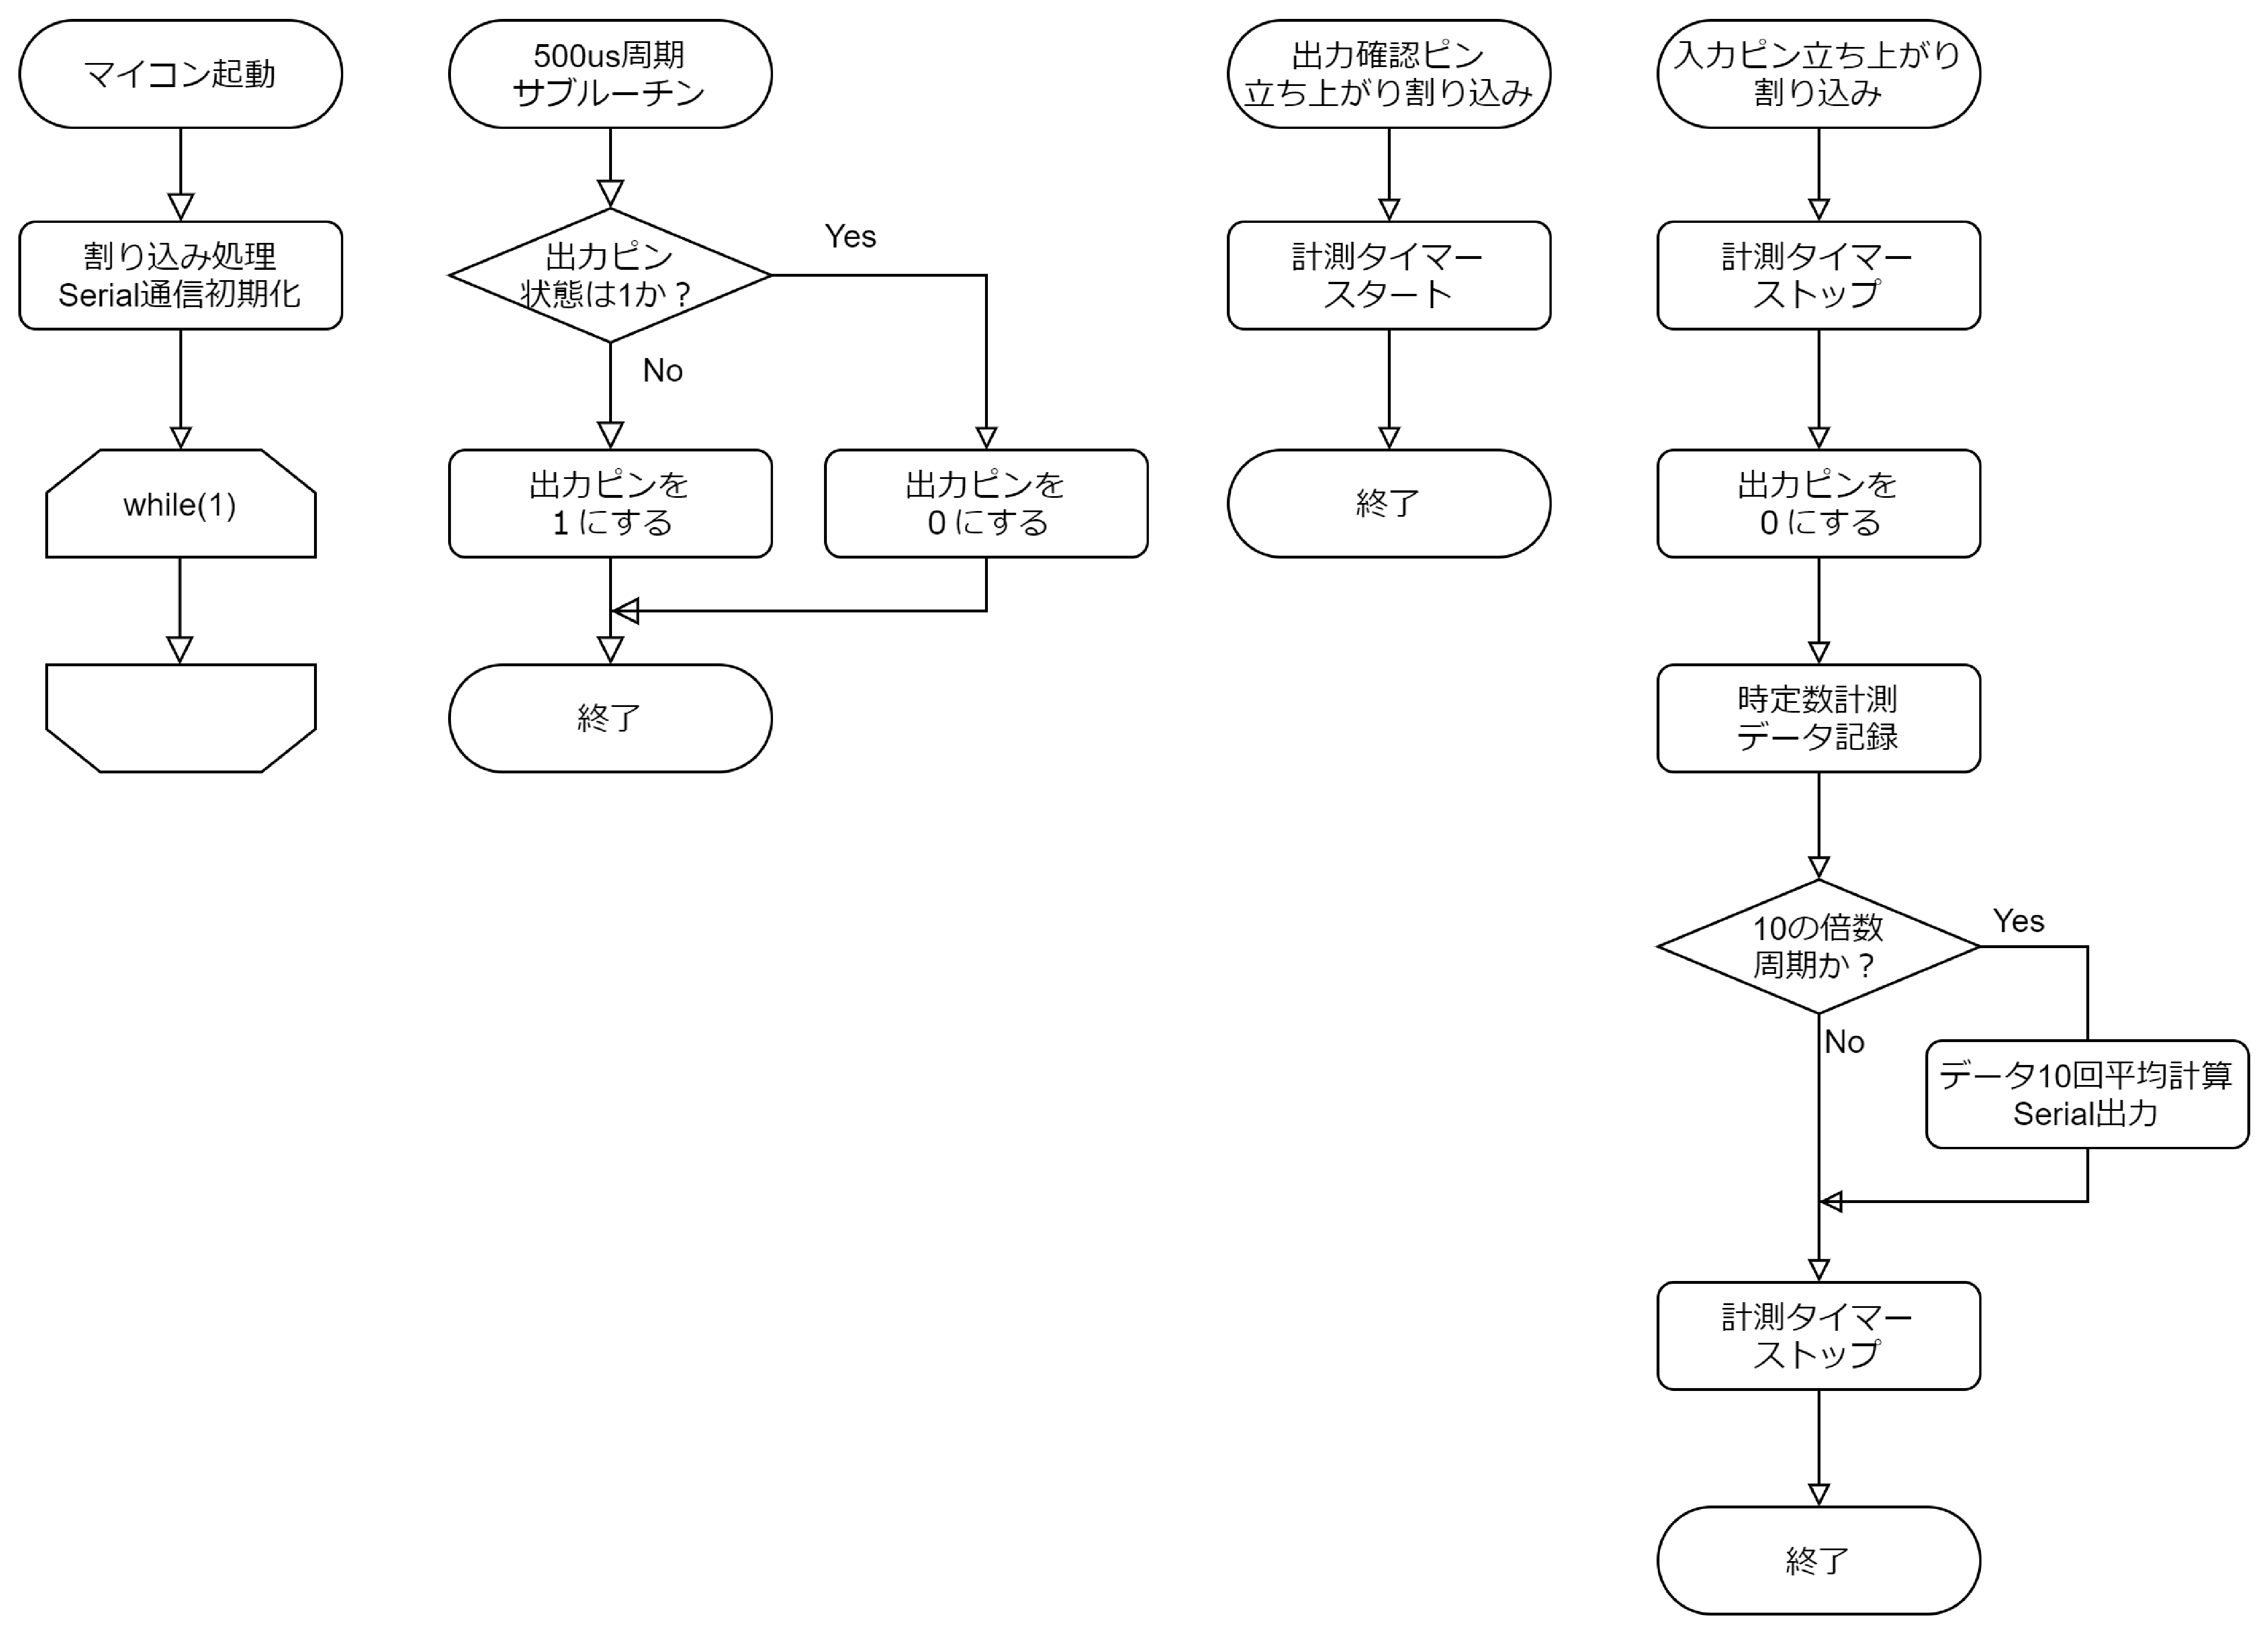
\includegraphics[width=0.9\columnwidth,clip]{./3_analysis/algorithm.eps}
     \caption{計測プログラムにおけるアルゴリズム}
     \label{fig:algorithm}
    \end{center}
\end{figure}

\section{足関節ロボット駆動システム}
足関節ロボットの駆動システムには従来から存在するペダリングロボット、2足歩行ロボットのシステムと同様のシステムを利用した

Visual Studio 2010 C++ を用いたMFCアプリケーションを用いた

空気圧電磁弁への電圧指令(0~550)を記述したtxtファイル読み込み

AD変換ボード

\section{フレキシブルストレッチセンサ計測データ処理}
